\begin{center}
    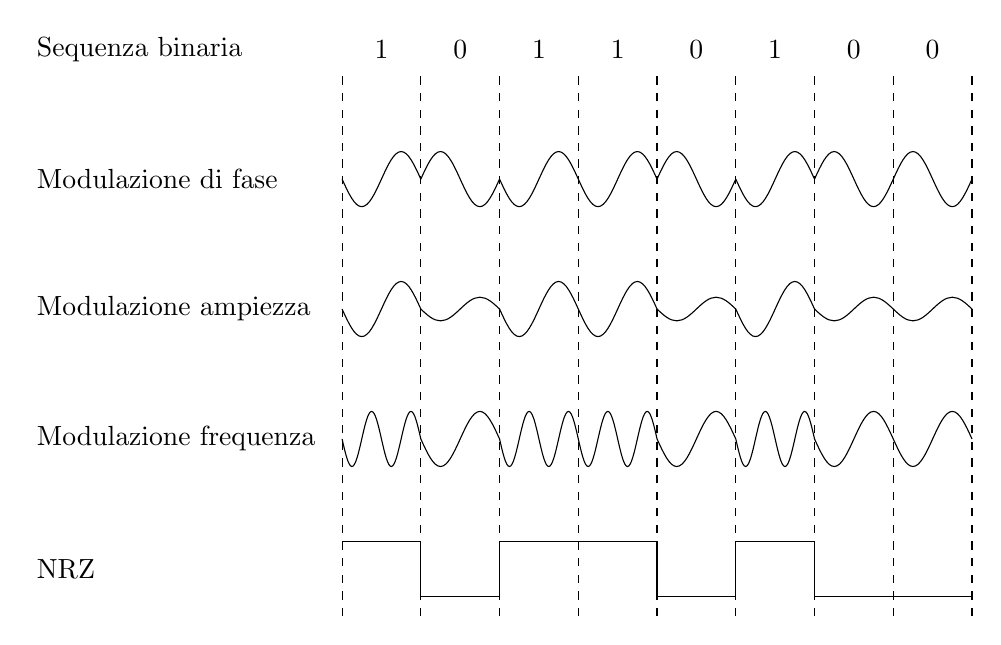
\begin{tikzpicture}
        %%%%%%%%% Barre %%%%%%%%%%
        \foreach \x in {4,...,12}
            \draw[dashed] (\x,-0.25) -- (\x,6.65);

        %%%%%%%%% Numeri %%%%%%%%%
        \node at (4.5,6.95) {1};
        \node at (5.5,6.95) {0};
        \node at (6.5,6.95) {1};
        \node at (7.5,6.95) {1};
        \node at (8.5,6.95) {0};
        \node at (9.5,6.95) {1};
        \node at (10.5,6.95) {0};
        \node at (11.5,6.95) {0};

        %%%%%%%%%% NRZ %%%%%%%%%%%
        \draw (4,.7) -- (5,.7) -- (5,0) -- (6,0) -- (6,.7) -- (8,.7) -- (8,0) -- (9,0) -- (9,.7) -- (10,.7) -- (10,0) -- (12,0);

        %%%%%%% Frequenza %%%%%%%%
        \draw (4,2) sin (4.125,1.65) cos (4.25,2) sin (4.375,2.35) cos (4.5,2) sin (4.625,1.65) cos (4.75,2) sin (4.875,2.35) cos (5,2);
        \draw (5,2) sin (5.25,1.65) cos (5.5,2) sin (5.75,2.35) cos (6,2);
        \draw (6,2) sin (6.125,1.65) cos (6.25,2) sin (6.375,2.35) cos (6.5,2) sin (6.625,1.65) cos (6.75,2) sin (6.875,2.35) cos (7,2) sin (7.125,1.65) cos (7.25,2) sin (7.375,2.35) cos (7.5,2) sin (7.625,1.65) cos (7.75,2) sin (7.875,2.35) cos (8,2);
        \draw (8,2) sin (8.25,1.65) cos (8.5,2) sin (8.75,2.35) cos (9,2);
        \draw (9,2) sin (9.125,1.65) cos (9.25,2) sin (9.375,2.35) cos (9.5,2) sin (9.625,1.65) cos (9.75,2) sin (9.875,2.35) cos (10,2);
        \draw (10,2) sin (10.25,1.65) cos (10.5,2) sin (10.75,2.35) cos (11,2) sin (11.25,1.65) cos (11.5,2) sin (11.75,2.35) cos (12,2);

        %%%%%%%% Ampiezza %%%%%%%%
        \draw (4,3.65) sin (4.25,3.3) cos (4.5,3.65) sin (4.75,4) cos (5,3.65) sin (5.25,3.5) cos (5.5,3.65) sin (5.75,3.8) cos (6,3.65) sin (6.25,3.3) cos (6.5,3.65) sin (6.75,4) cos (7,3.65) sin (7.25,3.3) cos (7.5,3.65) sin (7.75,4) cos (8,3.65) sin (8.25,3.5) cos (8.5,3.65) sin (8.75,3.8) cos (9,3.65) sin (9.25,3.3) cos (9.5,3.65) sin (9.75,4) cos (10,3.65) sin (10.25,3.5) cos (10.5,3.65) sin (10.75,3.8) cos (11,3.65) sin (11.25,3.5) cos (11.5,3.65) sin (11.75,3.8) cos (12,3.65);

        %%%%%%%%%% Fase %%%%%%%%%%
        \draw (4,5.3) sin (4.25,4.95) cos (4.5,5.3) sin (4.75,5.65) cos (5,5.3);
        \draw (5,5.3) sin (5.25,5.65) cos (5.5,5.3) sin (5.75,4.95) cos (6,5.3);
        \draw (6,5.3) sin (6.25,4.95) cos (6.5,5.3) sin (6.75,5.65) cos (7,5.3) sin (7.25,4.95) cos (7.5,5.3) sin (7.75,5.65) cos (8,5.3);
        \draw (8,5.3) sin (8.25,5.65) cos (8.5,5.3) sin (8.75,4.95) cos (9,5.3);
        \draw (9,5.3) sin (9.25,4.95) cos (9.5,5.3) sin (9.75,5.65) cos (10,5.3);
        \draw (10,5.3) sin (10.25,5.65) cos (10.5,5.3) sin (10.75,4.95) cos (11,5.3) sin (11.25,5.65) cos (11.5,5.3) sin (11.75,4.95) cos (12,5.3);

        %%%%%%%% Legenda %%%%%%%%%
        \node[anchor=west] at (0,6.95) {Sequenza binaria};
        \node[anchor=west] at (0,5.3) {Modulazione di fase};
        \node[anchor=west] at (0,3.65) {Modulazione ampiezza};
        \node[anchor=west] at (0,2) {Modulazione frequenza};
        \node[anchor=west] at (0,0.35) {NRZ};
    \end{tikzpicture}
\end{center}